% Presentation and notes for talk on
% Image Segmentation 2018 using Mask R-CNN
% Lecture: Seminar on Machine Learning, University of Regensburg
% Author: Gesina Schwalbe
% Supervisor: Justin Noel

\usepackage{fontspec}
\usepackage[shorthands=off]{babel}
\usepackage{csquotes}
\usepackage{lmodern}
\usepackage{graphicx}
\graphicspath{{./images/}}
\usepackage{mathtools,dsfont}
\usepackage{booktabs}
\usepackage[style=numeric, backend=biber]{biblatex}
\bibliography{image_segmentation.bib}




% titlepage
\title{Image Segmentation 2018}
\subtitle{with Mask R-CNN}
\author{Gesina Schwalbe}
\date{7th May 2018}
\mode<article>{
  \publishers{Seminar on Machine Learning, University of Regensburg\\
    Supervisor: Justin Noel}
}


\newcommand{\R}{\mathds{R}}
\newcommand{\IoU}{\text{\textbf{IoU}}}
\newcommand{\reg}{\textit{reg}}
\newcommand{\cls}{\textit{cls}}


\begin{document}

% title and table of contents
\frame{\maketitle}
\frame{\tableofcontents[hideallsubsections]}

% ------

\section{Definition and Goals}
\subsection{Problem}
\begin{frame}[<+->]
  \frametitle{General Goals}
  \mode<article>{The problem of image segmentation is to find}
  \begin{itemize}
  \item bounding boxes
  \item classification of each box
  \item pixel-mask for each box
  \end{itemize}
  \mode<article>{for a given image containing none, one, or several
    objects; if possible with more than 1fps.}
  \begin{block}{Datasets}
    \mode<article>{Some common datasets for the image segmentation
      task, mostly associated with a couple of specific official
      challenges, are}
    \begin{itemize}
    \item COCO % TODO link
    \item ImageNet % TODO link
    \end{itemize}
  \end{block}
\end{frame}

\begin{frame}[<only@+>][t]
  \frametitle{Applications}
  \begin{itemize}
  \item live detection of signs, obstacles in traffic
    (\href{images/mask_rcnn_demonstration.mp4}{example video})
  \item automatic street map enhancement
    \begin{figure}
      \centering
      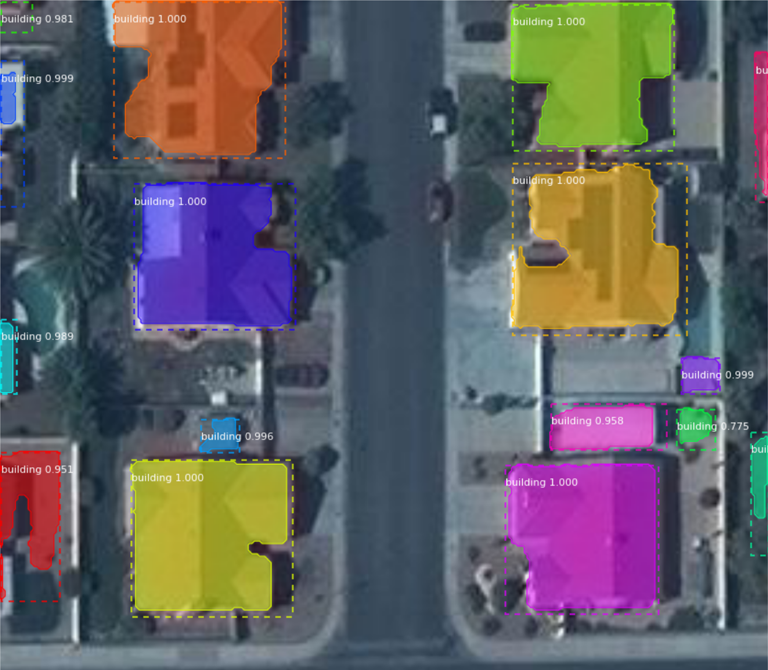
\includegraphics[width=0.5\textwidth]{mapping_challenge}
      \mode<article>{
        \caption{\href{https://github.com/crowdAI/crowdai-mapping-challenge-mask-rcnn}{Mapping
            Challenge solution}}
      }
    \end{figure}
  \item automatic evaluation of microscopy images
    \begin{figure}
      \centering
      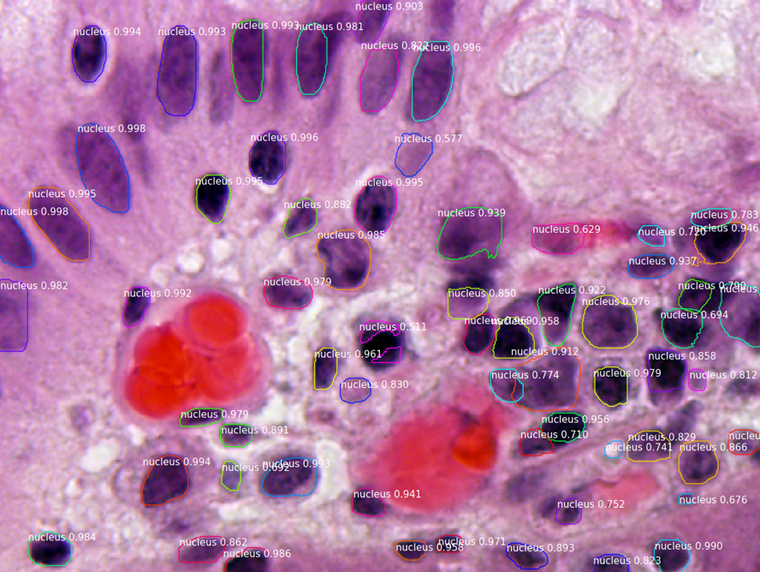
\includegraphics[width=0.5\textwidth]{nucleus_segmentation}
      \mode<article>{
        \caption{\href{https://github.com/matterport/Mask_RCNN/blob/master/samples/nucleus}{Nucleus
            segmentation}}
      }
    \end{figure}
  \end{itemize}
\end{frame}

\begin{frame}[<+->]
  \frametitle{Architectual Requirements}
  \begin{itemize}
  \item Master natural images: large nets
  \item Learn and process fast/efficiently\\
    (currently best: 32h wt. 8GPU learning; 5fps inference):
    \begin{itemize}
    \item special network components
      \mode<article>{instead of only fully connected layers}
      (CNN, ResNe(X)t, FPN)
    \item share many features (FPN, RPN)
    \item parallelize tasks/components
    \end{itemize}
  \end{itemize}
\end{frame}

\section{Architecture Components}
\subsection{Convolutional Networks}
\begin{frame}[<+->]
  \frametitle{What}
  \mode<article>{The main ingredient to convolutional networks,
    convolutional layers, are very good at detecting and summarizing
    local features in large data-spaces (e.g. corners, edges, patterns
    in images, i.e. self-learned image-preprocessing). The key
    features are
  }
  \begin{itemize}
  \item Feedforward neural network with only local connections
  \item Massive weight sharing
  \item (often:) Downscaling of feature space:
    \begin{itemize}
    \item Translation invariance
      \mode<article>{(see anchor boxes later)}
    \item Multiple scale feature spaces available
      \mode<article>{(see RPN anchor pyramid and FPN later)}
    \end{itemize}
  \end{itemize}
\end{frame}

\begin{frame}
  \frametitle{Convolution Operation}
  \mode<article>{
    The input space of a convolution is $\R^{n_1\times n_2\times
      \dotsb n_3}$.
    Each point (image) is a discrete ${n_1\times n_2\times
      \dotsb n_r}$ coordinate grid of values (pixels). The induced
    measure of distance of coordinates gives a notion of surrounding
    area for each coordinate.
    
    A convolution in machine learning is a}
  linear map $\R^{n_1\times n_2\times \dotsb n_3} \to \R^{n_1\times
    n_2\times \dotsb n_3}$ described by
  \begin{itemize}
  \item a fixed sliding window shape
    \mode<article>{i.e. a $k_1\times\dotsb k_r$
      grid (usually a square)}
  \item a window of that shape with a weight value at each coordinate,
    called the \emph{kernel}.
  \end{itemize}
  \mode<article>{
    The output at a coordinate is given by the scalar product of
    the values in the its surrounding box with the kernel.
    The border coordinates need special treatment (e.g. continuation
    by 0).
  }
  % \includegraphics[height=5em]{1D_convolution_layer.jpg}
  \pause
  \href{https://upload.wikimedia.org/wikipedia/commons/4/4f/3D_Convolution_Animation.gif}{(Animation)}
\end{frame}

\begin{frame}[<+->][t]
  \frametitle{Convolutional Layer}
  \mode<article>{A convolutional layer is effectively a locally
    connected layer (each output pixel gets input only from nearby
    input pixels) that heavily shares parameters.
    It consists of several convolution operations in parallel,
    each followed by an activation function (usually non-linear)
    that is applied to every pixel.}
  \begin{description}
  \item<only@+-+(7)>[Convolution Hyperparameters:]~
    \begin{itemize}
    \item size of kernel (= weight-window)%
      \mode<article>{, usually square 3x3 or 5x5}
    \item padding variant (= border treatment)%
      \mode<article>{, usually \enquote{same}, i.e. extend with 0
        s.t. output dim = input dim} 
    \item number of filters (= number of parallel convolutions)%
      \mode<article>{; perform $i$ convolutions in parallel producing a
        $i$-times larger output}
    \item stride (= downsampling rate)%
      \mode<article>{; skip all except every $i$th coordinate}
      \visible<+->{\begin{figure}
        \centering
        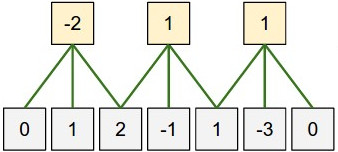
\includegraphics[width=0.5\textwidth]{1D_convolution_stride.jpg}
      \end{figure}}
    \item dilation (=upsampling rate)
      \mode<article>{; add $i$ virtual coordinates (wt. fixed value)
        inbetween}
    \item activation function \mode<article>{e.g. linear, ReLu}
    \end{itemize}
  \item<only@+>[Weights:] kernel values, bias
  \end{description}
\end{frame}

\begin{frame}[<+->]
  \frametitle{Pooling Layer}
  \mode<article>{
    Pooling is a way to downscale an image resp. summarize local sets
    of features. Given a window size, the input to the pooling
    layer is disected into windows of this size (with or without
    overlap) giving one output value per window calculated with a
    fixed operation, e.g. maximum or average. This reduces the number
    of features drastically, makes the network translation invariant
    up to the window size, and prevents overfitting to some extend.}
  
  Usual pooling functions
  \begin{itemize}
  \item Average Pooling (linear)
    \mode<article>{gives the average value of each window} 
  \item MaxPooling (non-linear)
    \mode<article>{gives the maximum value of each window}
    \visible<+->{\begin{figure}
      \centering
      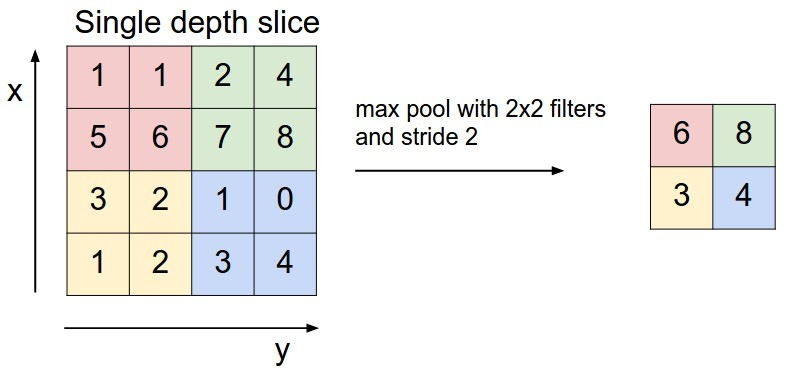
\includegraphics[width=.5\textwidth]{max_pooling.png}
      \mode<article>{\caption{2D-MaxPooling visualisation}}
    \end{figure}}
    \mode<article>{MaxPooling cheaply introduces one more non-linearity
      in the convolutional setup, and usually performs better than average
      pooling (Wikipedia).}
  \end{itemize}
\end{frame}

\subsection[Deep CNNs: ResNet and ResNeXt]{Deep CNNs: ResNet and
  ResNeXt}
For details see \cite{resnet}.
\begin{frame}
  \frametitle{(Deep) CNN}
  \mode<article>{A deep convolutional neural network (CNN or ConvNet)
    is a feedforward neural network consisting of:
    \begin{description}
    \item[Feature extraction backbone]
      stack of alternating
      \begin{itemize}
      \item convolutional layers, and
      \item pooling layers
      \end{itemize}
    \item[Feature interpretation]
      stack of fc neural network layers
      usually ending in a softmax layer for classification
    \end{description}
  }
  \begin{figure}
    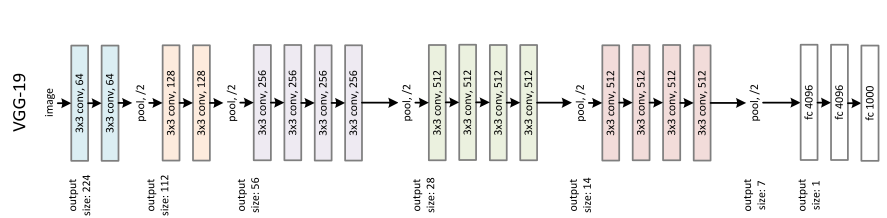
\includegraphics[width=\textwidth]{vgg.png}
    \mode<article>{
      \caption{VGG-19, a common ConvNet architecture developed by the
        Visual Geometry Group at Oxford University and predecessor of
        ResNet. Mind the alternating convolutional and pooling
        sections as well as the fully connected layers at the end.}
    }
  \end{figure}
\end{frame}

\begin{frame}
  \frametitle{Residual CNNs: ResNet}
  \mode<article>{Residual convolutional networks introduce identity
    shortcuts to circumvent the vanishing gradient problem of deep
    networks.
  }
  \only<+>{
    \begin{figure}
      \centering
      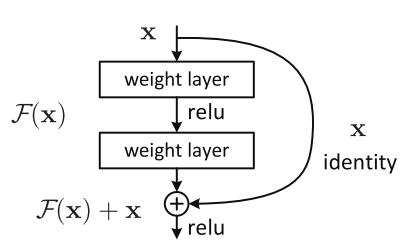
\includegraphics[width=0.7\textwidth]{residual_convnet_layer.png}
      \mode<article>{\caption{
          Residual component of a RCNN network. Up to two layers get a
          parallel identity shortcut
          \cite{resnet}.
        }}
    \end{figure}
  }
  \mode<article>{
    The actual trick is to provide alternative shorter \enquote{paths}
    for all weights. Intuitively this means that features detected in
    any stage are available in any other stage.}
  \only<+>{
    \begin{figure}
      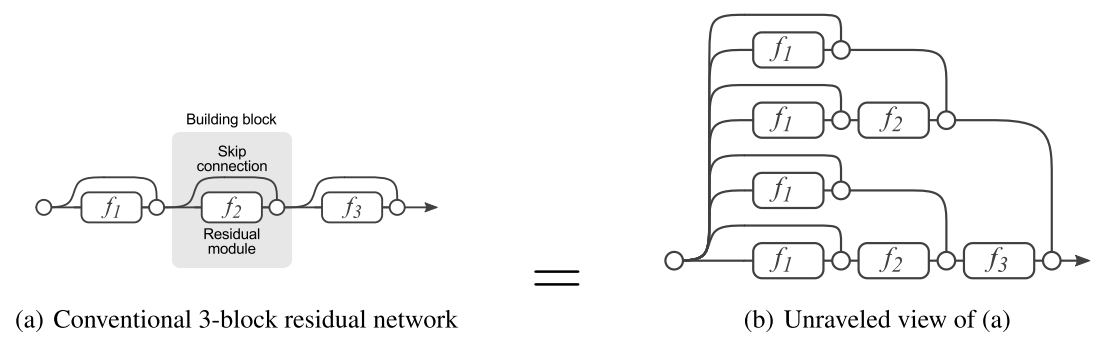
\includegraphics[width=\textwidth]{residual_convnet_layer-paths.png}
      \mode<article>{\caption{
          Impact of residual blocks within a network on paths through
          the network
          \cite{resnet}.
        }}
    \end{figure}
  }
\end{frame}

\begin{frame}
  \mode<article>{
    Best performance for residual modules was found for shortcutting 2
    stacks of linearity and non-linearity.
    ResNet is an example of a specific
    such network (usually 50 or 101 convolutional layers).
  }
  \begin{figure}
    \rotatebox{90}{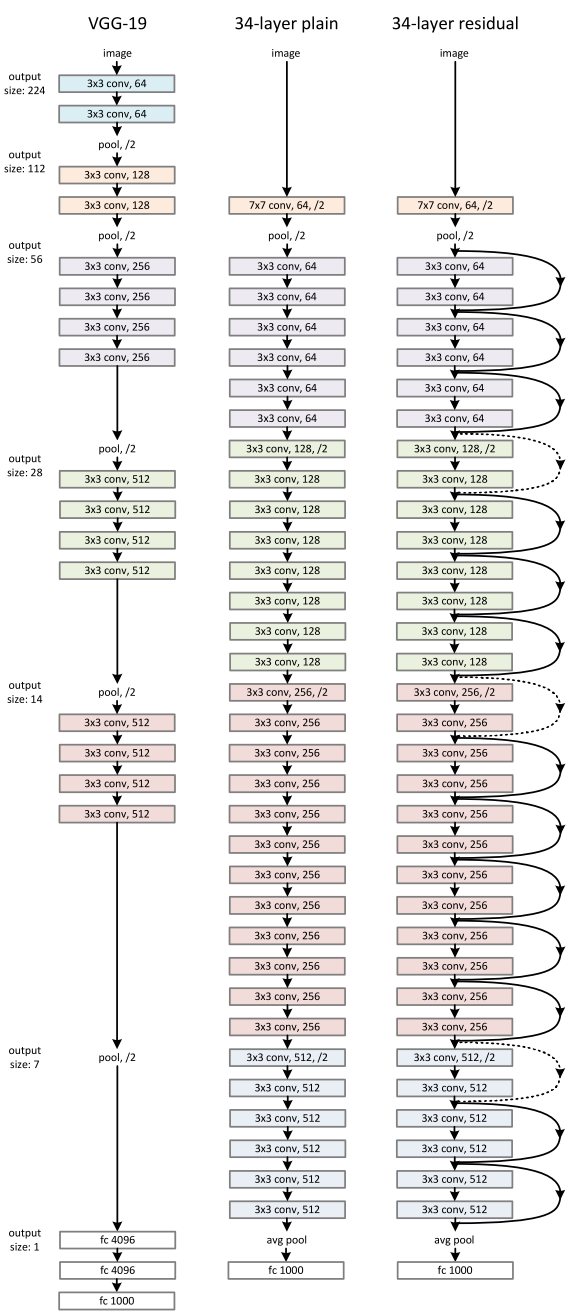
\includegraphics[height=\textwidth]{comparison_convnets.png}}
    \mode<article>{\caption{
        Comparison of VGG and ResNet: Residuals enable buiding much
        deeper convolutinal networks
        \cite{resnet}.
      }}
  \end{figure}
\end{frame}

\begin{frame}
  \mode<article>{
    ResNeXt splits the shortcutted parts into several parallel parts
    to get even more performance without further gradient vanishing.
  }
  \begin{figure}
    \centering
    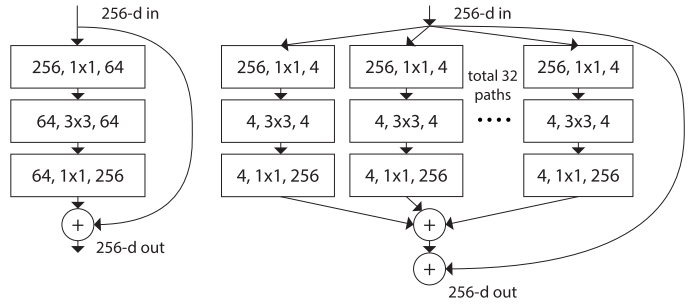
\includegraphics[width=0.7\textwidth]{resnext_convnet_layer.png}
    \mode<article>{\caption{
        Comparison of a normal residual block with one or
        ResNeXt. ResNeXt shortcuts many parallel branches
        \cite{resnet}.
      }}
  \end{figure}
\end{frame}

\begin{frame}
  \frametitle{More Feature sharing: FPNs}
  \mode<article>{
    Feature Pyramid Networks do not only use residuals to make earlier
    features more accessible in the final prediction block, but apply
    a prediction block at every feature stage. This makes the network
    more invariant to the scale of the feature to be detected.
  }
  \begin{figure}
    \centering
    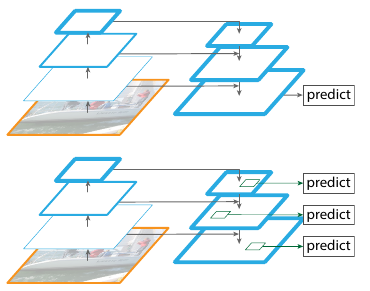
\includegraphics[width=0.6\textwidth]{fpn.png}
    \mode<article>{\caption{FPN setup principle}}
  \end{figure}
\end{frame}
\begin{frame}
  \begin{figure}
    \centering
    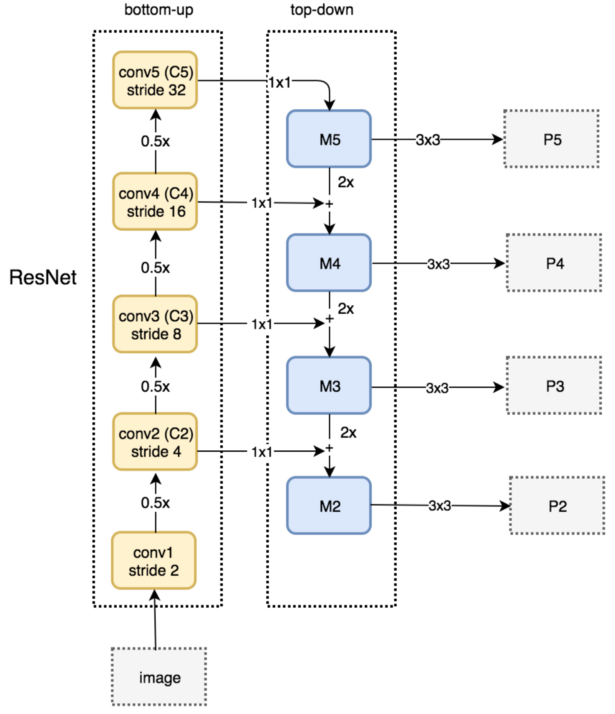
\includegraphics[width=0.6\textwidth]{fpn_with_resnet}
    \mode<article>{\caption{
        FPN with ResNet \cite{singleshotdetectors}
      }}
  \end{figure}
\end{frame}


\section{Model}
,\subsection{Overview}
\begin{frame}[<+->]
  \frametitle{Predecessor Problems}
  \begin{description}
  \item[Object Classification]
    \mode<presentation>{one object per image to one class per image}
    \mode<article>{Assume one object per image to classify.
      The key point here was to use sufficiently
      powerful architectures (FCNNs, ResNets, FPNs) to master the
      complexity of natural image features.}
  \item[Object Detection]~
    \begin{itemize}
    \item (intelligently) choose windows of the image
    \item classify each window \mode<article>{(including class "no obj")}
    \item maybe enhance the window selection
    \end{itemize}
    \mode<article>{The key point of Object Detection was to
      understand, that it can be done as a window-wise version of
      Object Classification. Main advances were how to effectively and
      efficiently choose the windows and how to share feature
      detection between overlapping windows.}
  \end{description}
\end{frame}

\begin{frame}[<+->]
  \frametitle{Components}
  \begin{enumerate}
  \item Convolutional backbone: extract important features
  \item Region proposal; \emph{in parallel:}
    \begin{itemize}
    \item Window objectness scoring
    \item Window correction
    \end{itemize}
  \item Frontend; \emph{in parallel:}
    \begin{itemize}
    \item Classification
    \item Masking
    \item Bounding Box Optimization
    \end{itemize}
  \end{enumerate}
\end{frame}

\subsection{Convolutional Backbone}
\begin{frame}
  \frametitle<presentation>{Convolutional Backbone}
  \begin{description}
  \item[Goal] extract features
  \item[Architecture]
    \mode<presentation>{same as for Object Detection}
    \mode<article>{The architecture should be chosen as for a
      convolutional backbone of an analogous Object Detection task,
      e.g. ResNet with FPN for natural image processing. See \ref{backbonetraining}.}
  \end{description}
\end{frame}

\subsection{Region Proposal Network}
\begin{frame}[<+->]
  \frametitle{Predecessors/Alternatives}
  \mode<article>{See \cite{regionproposaloverview} for a more detailed overview.}
  \begin{description}
  \item[Pixel Merging] (e.g. SelectiveSearch)
    \mode<article>{Merge pixels with neighbors to objects by
      manual or learned rules, starting at more or less
      intelligently chosen starting pixels.
      The computation is usually very costful.}
  \item[Window scoring] (e.g. Objectness)
    \mode<article>{Obtain a fixed or preselected set of candidate
      windows and learn/apply an objectness scoring algorithm.
      The localisation accuracy is usually low and the cost is
      proportional to the number of window candidates.
      Scale invariance is usually ensured by conducting the process
      several times for differently sized windows/image resize scales.}
  \item[Separate NN] (e.g. Multibox)
    \mode<article>{Separately train a complete neural network for
      region proposals. Usually very costful to train.}
  \end{description}
\end{frame}

\begin{frame}[<+->]
  \frametitle{Main Ideas of the Mask-RCNN Approach}
  Window scoring with enhancements:
  \begin{description}[]
  \item[Decoupling] of classification and window proposals
  \item[All Scales at once] using different candidate window shapes
  \item[Bounding box correction] in \emph{parallel} to scoring 
  \item[Excessive weight sharing] amongst same shapes
  \item[RoI-Pooling = Feature sharing] i.e. use convolutional features
    from backbone and pool each proposal window to fixed size
  \end{description}
\end{frame}

\begin{frame}[t]
  \frametitle{Architecture Overview}
  \begin{description}[<only@+->]
  \item[Shared Conv Layer]
    Sliding window on feature space
    with fixed set of anchor shapes per window
    \mode<article>{(=base box shape proposals)}
    \only<.>{
      \begin{figure}
        \centering
        \hbox{
          \parbox[c]{0.3\textwidth}{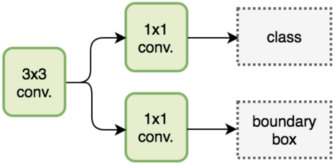
\includegraphics[width=0.3\textwidth]{rpn_components}\hbox{}}~
          \parbox[c]{0.65\textwidth}{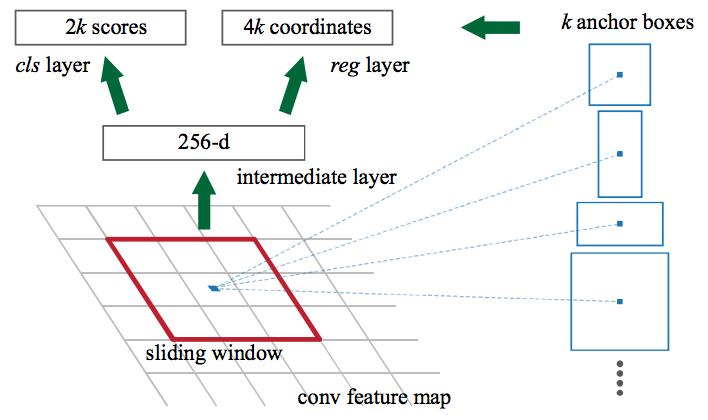
\includegraphics[width=0.65\textwidth]{anchors}\hbox{}}
        }
        \mode<article>{\caption{
            Left: RPN components \cite{singleshotdetectors};
            Right: Anchor shapes per center point i.e. feature map pixel
            \cite{fasterrcnn}.
          }}
      \end{figure}
    }
  \item[\cls{}, \reg{}] Per window and anchor shape do in parallel
    \begin{description}
    \item[objectness score] (\cls{})
      \mode<article>{This is analogous to the window scoring method
        and provides the rough region proposals. The main difference
        is the high weight sharing: Anchors of the same shape share
        their scoring algorithm, thus ensuring high translation
        invariance (it does not matter, in which corner of the image
        the object is) and high scale invariance (choose anchor shapes
        of different scale).}
    \item[coordinate correction] (\reg{})
      \mode<article>{This part tries to overcome the low localisation
        accuracy of usual window scoring and thus enables to use much
        less candidate windows (anchors), as only the aspect ration
        has to fit very roughly.}
    \end{description}
    \only<.>{
      \begin{figure}
        \centering
        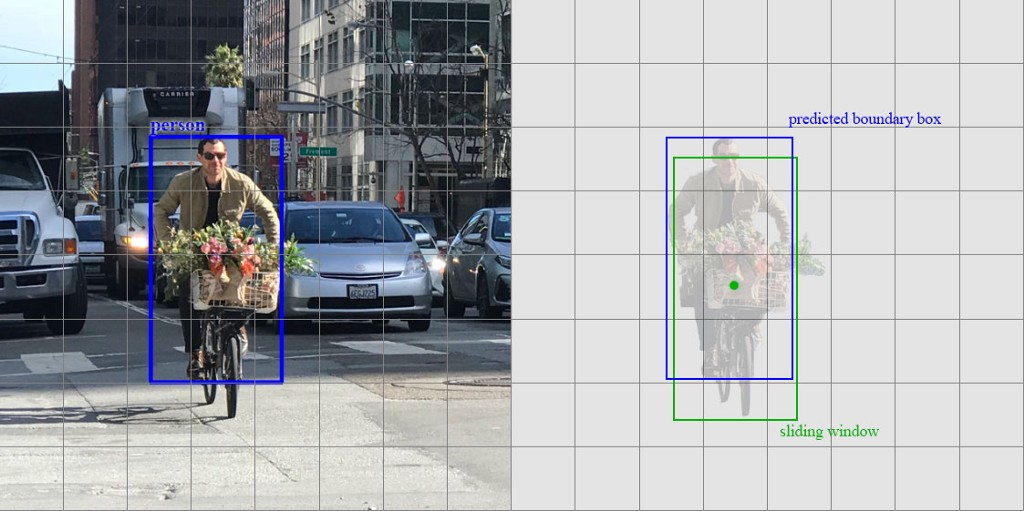
\includegraphics[height=0.3\textwidth]{rpn_reg_example}
        \mode<article>{\caption{
            Example of a bounding box correction by the \reg{} part
            of a region propsal network.
            \cite{singleshotdetectors}
          }}
      \end{figure}
    }
    \mode<article>{The main idea behind this parallel approach is,
      that with a well enough feature space output of the backend the
      questions
      \begin{itemize}
      \item \emph{Is} there an object of roughly that shape?
      \item If it was an object, what \emph{exact shape} would it have?
      \end{itemize}
      can actually be answered independently and also independent of
      the later object classification (class-agnostic region proposals).
    }
  \item[Proposal Layer] Select best proposals
  \end{description}
\end{frame}

\begin{frame}
  \begin{figure}
    \centering
    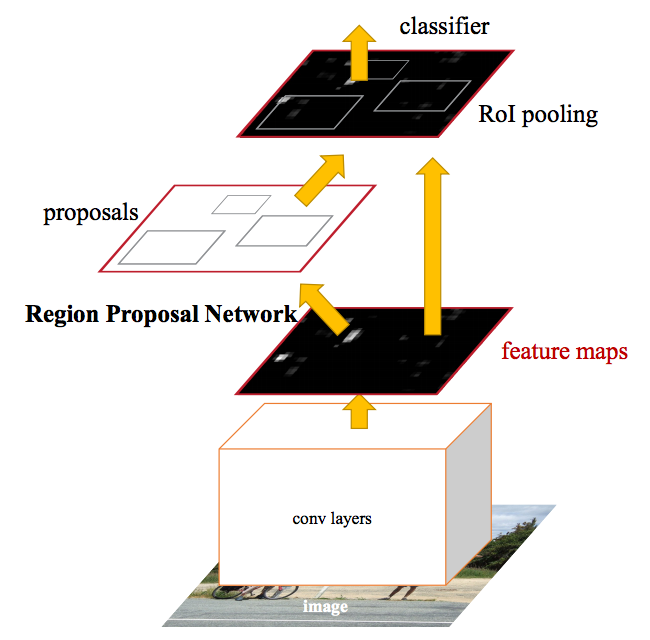
\includegraphics[width=0.7\textwidth]{rpn_in_network}
    \mode<article>{\caption{
        Location of the RPN component within the network
      }}
  \end{figure}
\end{frame}

\begin{frame}[t]
  \frametitle{Coordinate and RPN \reg{} output encoding}
  \mode<article>{All box coordinates are normalized,
    i.e. $x=\dfrac{x}{\text{image\_width}}$,
    $y=\dfrac{y}{\text{image\_height}}$.}
  \begin{description}[<only@+>]
  \item[Box coordinate] encoding (all normalized):
    \begin{itemize}[<.->]
    \item[$(x_1,y_1$] \texttt{\# \small upper left corner}
    \item[$x_2,y_2)$] \texttt{\# \small lower right corner}
    \end{itemize}
    
  \item[Coordinate correction] (=\reg{} output) encoding:
    \begin{itemize}[<.->]
    \item[$\Big(dx,$]
      \texttt{\# \small $\frac
        {\text{centerpoint x-difference}}
        {\text{anchor width}}$}
      $\phantom{\Big|}$
    \item[$dy,$]
      \texttt{\# \small $\frac
        {\text{centerpoint y-difference}}
        {\text{anchor height}}$}
      $\phantom{\Big|}$
    \item[$\log(dw),$]
      \texttt{\# \small $\frac
        {\text{ground-truth box width}}
        {\text{anchor width}}$}
      $\phantom{\Big|}$
    \item[$\log(dh)\Big)$]
      \texttt{\# \small $\frac
        {\text{ground-truth box height}}
        {\text{anchor height}}$}
    \end{itemize}
  \end{description}
\end{frame}

\begin{frame}
  \frametitle<presentation>{Metrics}
  \mode<article>{The metric for measuring how well a proposal window
    fits for a real bounding box is the \emph{intersection over union
      ratio (IoU)}. For two measurable subsets $A$, $B$ of $\R^2$ this
    is defined as}
  \mode<presentation>{Metric for matching:}
  \begin{gather*}
    \IoU(A, B) \coloneqq \dfrac{\text{Intersection Area}}{\text{Union Area}}
  \end{gather*}
  % TODO: IoU visualization?
\end{frame}

\begin{frame}[<+->]
  \frametitle{Labels}
  \mode<article>{For each anchor we assign an objectness label, and
    if this is positive, a corresponding ground-truth bounding box
    (else the ground-truth bounding box is set to all 0):}
  \begin{description}[-1=no object]
  \item[object=1] with ground-truth box $b$ if
    \begin{itemize}
    \item \mode<article>{it has the} best $\IoU$ for $b$, else if
    \item $\IoU$ with $b$ $\geq$ 0.3
    \end{itemize} 
  \item[no object=-1] if not pos. and $\IoU\leq 0.3$
  \item[neutral=0] else (excluded from training)
  \end{description}
  \mode<article>{All neutral boxes get completely excluded from
    training resp. from the loss calculation.}
  Balance positive and negative boxes for training!
  \mode<article>{This can e.g. be done by setting most of the actually
    negative anchors to neutral to be excluded from training.}
\end{frame}

\begin{frame}[t]
  \frametitle{Architecture Details}
  \begin{description}[<only@+>]
  \item[Sliding window]
    \mode<presentation>{Shared Conv layer with \enquote{valid}-padding}
    \mode<article>{This is implemented by a shared convolutional
      layer that naturally gives one value per sliding window (=kernel
      location). The padding is \enquote{valid} to exclude anchors
      crossing image borders (see \reg{}-Training).}
  \item[Objectness classification] Conv layer with
    \begin{itemize}[<.->]
    \item $1\times1$-sized kernel
    \item 2-class softmax activation:
      (non-object score, object score)
    \end{itemize}
    \emph{Loss:} crossentropy for non-neutral anchors
  \item[Coordinate correction]
    Conv layer with
    \begin{itemize}[<.->]
    \item $1\times1$-sized kernel
    \item $4\times\text{(number of anchors)}$ filters:
      $(dx,dy,dw,dh)$ coordinate correction for each anchor
    \end{itemize}
    \emph{Loss:} smooth $L_1$-loss\mode<article>{\footnote{
        The smooth $L_1$-loss takes the smoothed out absolute value
        \begin{gather*}
          |d|_\text{smooth} \coloneqq \begin{cases}
            0.5 \cdot d^2 & \text{d=1}\\
            |d|_1 & \text{d>1}
          \end{cases}
        \end{gather*}
        This is differentiable and the loss is more robust to
        outliers than $L_2$.
      }}
    for positive anchors that do not cross image bounds
    \mode<article>{\par
      The border-crossing anchors are excluded because:
      \begin{quote}
        [They would] introduce large, difficult to correct error terms in
        the objective, and training does not converge.
      \end{quote}
      This is simply implemented by a \enquote{valid}-padding for the
      sliding window; or alternatively setting their ground-truth
      objectness score to neutral (thus they are ignored during
      training, see \cls{}-Training).
    }
  \item<only@+->[Proposal selection]~
    \begin{enumerate}[<+->]
    \item Trim to $N$ best-object-scored anchors.
    \item Apply coordinate correction.
    \item Clip boxes.
      \mode<article>{This is necessary, because the coordinate
        corrections may well exceed the sliding window size, in which
        the original anchor lies. This makes sense, because one can
        suggest the size of an object without seeing it resp. its
        surroundings completely. However, anchors at the }
    \item Non-maximum suppression:
      \begin{enumerate}
      \item Sort by score
      \item Reject boxes which have high IoU with better scored ones
      \item Trim to best \emph{num\_proposals}
      \end{enumerate}
    \end{enumerate}
  \end{description}
\end{frame}

\subsection{RoI-Pooling}
Region of Interest (RoI) pooling is the process of
resizing the output of a proposed window to the frontends input
shape.
This is done by uniformly splitting the window into rectangular
regions, one for each desired output pixel, and pooling each
rectangle to this one pixel. As this means downscaling, all of the
window outputs have to be larger than the frontend's input shape.
\begin{frame}
  \frametitle<presentation>{RoI-Pooling}
  \begin{figure}
    \mode<presentation>{
      \parbox[c]{0.5\textwidth}{
        \only<+>{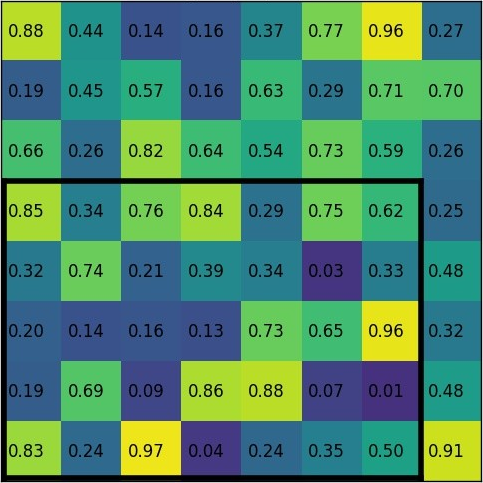
\includegraphics[scale=0.3]{roipooling1-cropped}}%
        \only<+->{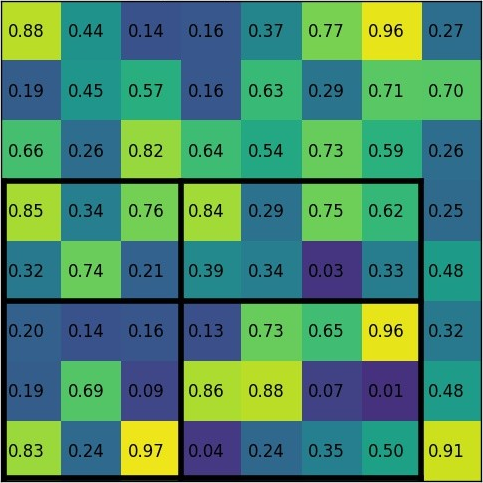
\includegraphics[scale=0.3]{roipooling2-cropped}}%
        \hbox{}
      }
      \parbox[t]{0.2\textwidth}{\visible<+->{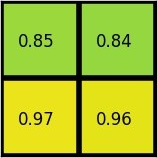
\includegraphics[scale=0.3]{roipooling3-cropped}}\hbox{}}
    }
    \mode<article>{
      \begin{center}
        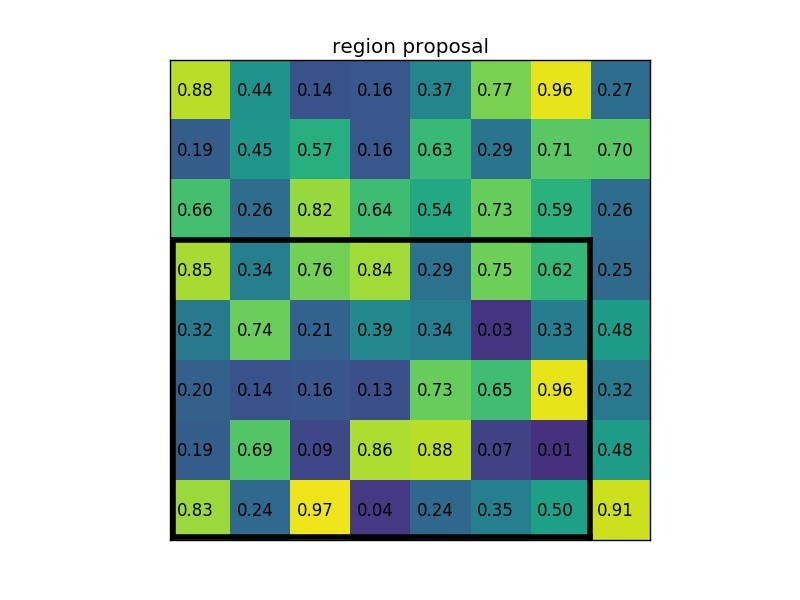
\includegraphics[scale=0.3]{roipooling1}
        
        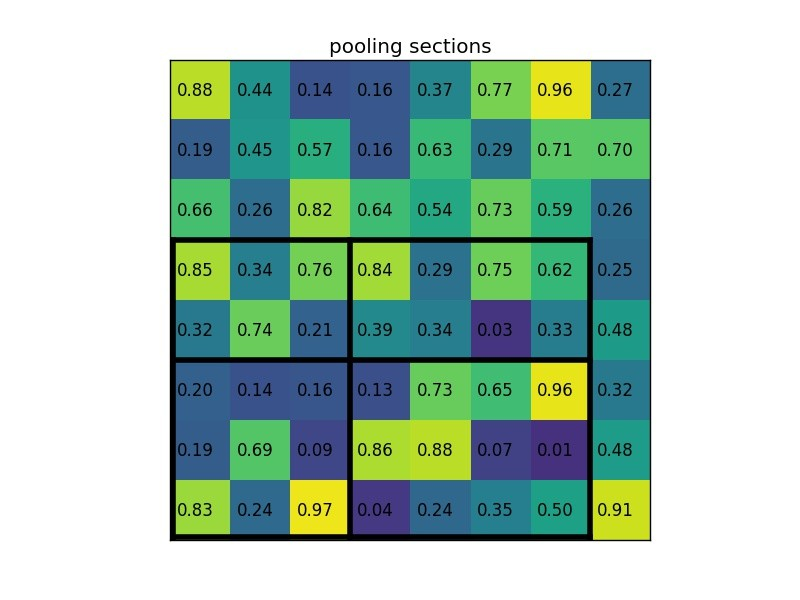
\includegraphics[scale=0.3]{roipooling2}

        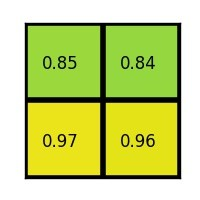
\includegraphics[scale=0.3]{roipooling3}
        \caption{
          Visualization of Region of Interest Pooling.
          From top to bottom: Selection of a window; splitting of the
          window into roughly equal rectangular sections (round half
          width/height to full pixels); Max-Pooling output of the segmentation
        }
      \end{center}
    }
  \end{figure}   
\end{frame}

\begin{frame}
  \frametitle{RoI-Align}
  \mode<presentation>{Bilinear interpolation instead of cropping:}
  
  \mode<article>{RoI-align suggests to avoid any cropping/rounding
    when disecting the windows output into rectangles for
    pooling. This can be done by calculating the rectangle values via
    bilinear interpolation instead of cropping to full pixels followed
    by e.g. average pooling.
    Using RoI-Align, the feature maps from the bounding boxes
    evaluated by the frontend are more accurately aligned with the
    original image and masks get better.}
  \begin{figure}
    \centering
    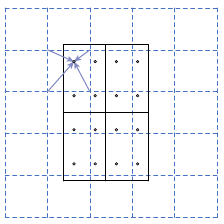
\includegraphics{roialign}
    \mode<article>{\caption{
        Visualization of RoI-Align: A pixel on the output feature map
        is bilinearly interpolated from nearby pixels in the input
        feature map.
      }}
  \end{figure}
\end{frame}

\subsection{Frontend}
\begin{frame}[<+->]
  \frametitle{Main Ideas}
  Decouple
  \begin{itemize}
  \item classification, bounding box optimization, and masks;
  \item mask predictions for the different classes
  \end{itemize}
\end{frame}


\begin{frame}[t]
  \frametitle{Architecture}
  \only<+>{
    \begin{figure}
      \centering
      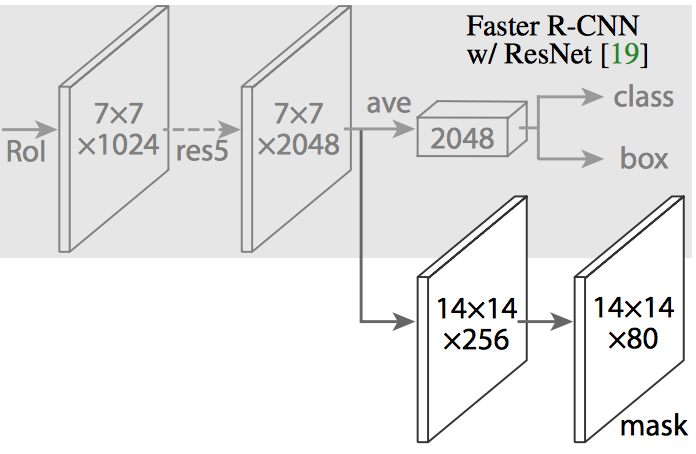
\includegraphics[width=0.7\textwidth]{frontend}
      \mode<article>{\caption{
          Frontend architecture overview;
          in this case a ResNet-FPN backend is assumed.
          Note the three mostly independent prediction branches.
        }}
    \end{figure}
  }
  \begin{description}[<only@+>]
  \item[Classification]
    fully connected layers ending in softmax
    (include class \enquote{No object})%
    \mode<article>{\par
      The network should look like the network head used for the
      corresponding object detection task, see Backbone Pretraining.
    }
    \emph{Loss:} multinomial crossentropy
  \item<only@+>[Mask generation]~
    \begin{enumerate}[<.->]
    \item Few (1--3) Conv Layers,
      maybe with upscaling parts
    \item Conv Layer with
      \begin{itemize}
      \item a filter for each class
      \item sigmoid activation
      \end{itemize}
      \mode<article>{This means, as for the RPN, classification and
        mask (=per pixel scoring) are handled independently.
        Tests showed, this works much better than sharing filters for
        all classes and apply a softmax with multinomial cross-entropy
        loss, because here mask results from several classes influence
        each other
        \cite{maskrcnn}.
      }
    \end{enumerate}
    \emph{Loss:} binary cross-entropy
  \item[Bounding box regression] Linear regression
  \end{description}
\end{frame}


\section{Training}
\subsection{Overview}
\begin{frame}[<+->]
  \frametitle<presentation>{Steps}
  \mode<article>{Even though the training could be conducted on the
    complete network at once, this is not advisable as the different
    components would influence each other heavily. Thus training is
    splittet in several steps:}
  \begin{enumerate}
  \item Backbone
  \item RPN
  \item Alternating training of RPN and Frontend
  \end{enumerate}
\end{frame}

\subsection{Backbone Pretraining}\label{backbonetraining}
\begin{frame}[<+->][t]
  \frametitle<presentation>{Backbone Pretraining}
  \mode<article>{To train the backbone, a separate ConvNet model is
    set up with the convolutional backbone to train as backbone and a
    fully connected frontend.} 
  \begin{block}{Separate ConvNet Training Model}
    \begin{enumerate}
    \item Backbone (Conv \& Pooling)
    \item Dense Layers
    \item Classification Softmax-Layer
      \mode<article>{Here the \enquote{No object} class should already
        be respected and trained.}
    \end{enumerate}
  \end{block}

  \begin{block}{Training Input}
    \begin{description}
    \item[inputs] one-object images
      (ca. size of later bounding boxes)
    \item[labels] the single objects' labels
    \end{description}
  \end{block}
\end{frame}

\subsection{Alternating Training}
\begin{frame}[<+->]
  \frametitle<presentation>{Alternating Training}
  \mode<article>{One further special thing about image segmentation
    with a region proposal network is the preferable training routine,
    where region proposal network and the frontend are trained
    alternately. The proposed order is:
  }
  (after RPN is trained)
  \begin{enumerate}
  \item Frontend: RPN fixed, backbone not shared
  \item RPN: frontend fixed, shared backbone fixed
  \item Frontend: RPN fixed, shared backbone fixed
  \item \dots \mode<article>{(not much further improvement with more
      repetitions)}
  \end{enumerate}
\end{frame}

\section*{Implementation Review}
\subsection{Source Code}
\begin{frame}
  \frametitle<presentation>{Example Sources}
  \begin{itemize}
  \item
    \href{https://github.com/matterport/Mask_RCNN/blob/master/samples/demo.ipynb}
    {Keras implementation by matterport}: \cite{maskrcnnkeras}
  \item Easy example for handwritten number detection using
    autogenerated data based on MNIST: \href{https://github.com/gesina/simple_mask_rcnn}{github}
  \end{itemize}
\end{frame}

\begin{frame}[<+->]
  \frametitle{Keras Implementation Specialties}
  \begin{itemize}
  \item Use the functional API!
  \item Custom layers:
    \begin{description}[<.->][RoI-Pooling Layer]
    \item[Loss Layers] custom losses
    \item[Proposal Layer] select RPN proposals
    \item[RoI-Pooling Layer] reshape proposals and mask labels
      (can use
      \href{https://www.tensorflow.org/api_docs/python/tf/image/crop_and_resize}
      {\texttt{tf.crop\_and\_resize()}})
    \end{description}
  \item Separate models for training and inference
    \mode<article>{Since in keras a specified loss will be applied to
      all outputs, one needs to use the more internal
      \texttt{model.add\_loss()} function as a workaround.
      This function accepts a layer whose output will be added to the
      overall loss.
      As the loss layers need the ground-truth labels as inputs, one
      has to define separate models for training and inference.}    
  \end{itemize}
\end{frame}

\subsection{Lessions learned}
\begin{frame}[allowframebreaks]
  \frametitle<presentation>{Lessions Learned}
  \begin{itemize}
  \item Always double-check and note down tensor/array dimensions;
    mind the padding for convolutions.
  \item Always double-check and test your algorithms.
  \item Always have a look at \emph{all} input and output data:
    \begin{itemize}
    \item Do they roughly make sense, e.g. do positive classes have
      different probability output than negative ones?)
    \item Are there error patterns?
    \end{itemize}
    Visualization is your friend. But it will contain bugs, too.
  \item Directly document and update all input and output formats of
    functions. Resp. in general: Keep your code VERY clean and understandable.
  \item Convolution is very geometric: Depict your sliding windows and
    downscaling factor(s) to check whether they make sense with your
    data/object sizes.
  \item Mind your RAM when optimizing data generation/tagging
  \item Check your loss and validation values; Does the model actually
    get better?
  \item The deeper, the much more time;
  \item Make data as easy (small) as possible; if you can still
    classify, the network can do, too (e.g. grayscale instead of several
    color channels).
  \end{itemize}
\end{frame}

\nocite{*}
\printbibliography[heading=none]

\end{document}

%%% Local Variables:
%%% mode: latex
%%% TeX-master: "image_segmentation-beamer"
%%% End:
